\input{head.inc}
 \usetikzlibrary{overlay-beamer-styles}
  
% Präambelbefehle für die Präsentation
\title[TET: Elektromagnetische Wellen VII - Allgemeine Lösung]{Elektromagnetische Wellen VII - Allgemeine Lösung}

\begin{document}
% 
% Frontmatter 
% 
%%%%%%%%%%%%%%%%%%%%%%%%%%%%%%%%%%%%%%%%%%%%%%%%%%%%%%%%%%%%%%%%%%%%%%%%%%%%%%%%%%%%%%%%%%%%%%%%%%%%%%%%%%%%%%%%%%%%%%%%%%%%% 

%% inserts the title page and the table of contents
\maketitle

% 
% Content 
% 
%%%%%%%%%%%%%%%%%%%%%%%%%%%%%%%%%%%%%%%%%%%%%%%%%%%%%%%%%%%%%%%%%%%%%%%%%%%%%%%%%%%%%%%%%%%%%%%%%%%%%%%%%%%%%%%%%%%%%%%%%%%%% 
\section{Elektromagnetische Wellen VII - Allgemeine Lösung}

\begin{frame}
  \frametitle{Ausgangspunkt}
  \begin{itemize}[<+->]
  \item Wir suchen die \alert{allgemeine Lösung} \(\Psi(\ortsvektor[v],t)\) der \alert{homogenen Wellengleichung} mit \alert{Anfangswerten} \(\Psi_0(\ortsvektor[v])\) und \(\dot{\Psi}_0(\ortsvektor[v])\):
    \begin{align*}
      \square\Psi(\ortsvektor[v],t) &= \left(\laplace - \varepsilon\mu\frac{\d^2}{\d t^2}\right)\Psi(\ortsvektor[v],t) = \left(\laplace - \frac{1}{\geschw_c^2}\frac{\d^2}{\d t^2}\right)\Psi(\ortsvektor[v],t) = 0\\
      \Psi(\ortsvektor[v],t=0) &= \Psi_0(\ortsvektor[v]) \text{ vorgegeben}\\
      \left.\frac{\d \Psi(\ortsvektor[v],t)}{\d t}\right|_{t=0} &= \dot{\Psi}_0(\ortsvektor[v]) \text{ vorgegeben}
    \end{align*}
  \item Diese allgemeine Lösung lässt sich durch \alert{Fourier-Transformation} der partiellen Differentialgleichung finden.
    \end{itemize}
  \end{frame}


 \begin{frame}
  \frametitle{Fourier-Transformation}
  \begin{block}{Definition}
    Es sei \(f: \mathbb{R}^n \to \mathbb{R}^n\) eine integrierbare Funktion (\(f \in L^1(\mathbb{R}^n\))). Dann ist die \alert{Fourier-Transformierte}${\mathcal F}$ von \(f\) definiert durch
    \begin{equation*}
      ({\mathcal F}f)(\vec{y}) = \tilde{f}(\vec{y}) = \int_{\mathbb{R}^n} f(\vec{x}) \euler^{-\komplex \vec{x}\cdot\vec{y}} \upd^n x \pointspacep
    \end{equation*}
    Die \alert{Rücktransformation} ${\mathcal F}^{-1}$ ist dann
    \begin{equation*}
      f(\vec{x}) = ({\mathcal F}^{-1} ({\mathcal F}f)(\vec{y}))(\vec{x}) = \frac{1}{(2\pi)^n} \int_{\mathbb{R}^n} \tilde{f}(\vec{y}) \euler^{\komplex \vec{x}\cdot\vec{y}} \upd^n y \pointspacep
    \end{equation*}
    \end{block}
  \begin{itemize}[<+->]
    \item Produkt der Faktoren bei Hin- und Rücktransformation muss \(\frac{1}{(2\pi)^n} \) ergeben und die Vorzeichen der Exponentialfunktionen sind unterschiedlich!
    \item Konvention: Für das Paar \(t \leftrightarrow \omega\) wird das jeweils entgegengesetzte Vorzeichen in der Exponentialfunktion verwendet.
      \item Wichtige Regeln: \alert{Faltungssatz}, \alert{Verschiebungssatz}, \alert{Darstellung der \(\delta\)-Funktion}
    \end{itemize}
  \end{frame}
 

 \begin{frame}
  \frametitle{Zurück zur allgemeinen Lösung}
  \begin{itemize}[<+->]
  \item Wir suchen die \alert{allgemeine Lösung} \(\Psi(\ortsvektor[v],t)\) der \alert{homogenen Wellengleichung} mit \alert{Anfangswerten} \(\Psi_0(\ortsvektor[v])\) und \(\dot{\Psi}_0(\ortsvektor[v])\):
    \begin{align*}
      \square\Psi(\ortsvektor[v],t) &= \left(\laplace - \varepsilon\mu\frac{\d^2}{\d t^2}\right)\Psi(\ortsvektor[v],t) = \left(\laplace - \frac{1}{\geschw_c^2}\frac{\d^2}{\d t^2}\right)\Psi(\ortsvektor[v],t) = 0\\
      \Psi(\ortsvektor[v],t=0) &= \Psi_0(\ortsvektor[v]) \text{ vorgegeben}\\
      \left.\frac{\d \Psi(\ortsvektor[v],t)}{\d t}\right|_{t=0} &= \dot{\Psi}_0(\ortsvektor[v]) \text{ vorgegeben}
    \end{align*}
  \item Die Fourier-Transformierte der noch unbekannten Lösung sei \(\tilde{\Psi}(\wellenzahl[v], \omega)\)
  \item Hiermit schreiben wir \(\Psi(\ortsvektor[v], t)\) als \alert{Überlagerung ebener Wellen} mit beliebigen Wellenvektoren \(\wellenzahl[v]\) und Kreisfrequenzen \(\omega\)
    \begin{equation*}
      \Psi(\ortsvektor[v], t) = \frac{1}{(2\pi)^4} \iiint_{\mathbb{R}^3} \int_{-\infty}^\infty \tilde{\Psi}(\wellenzahl[v], \omega) \euler^{\komplex(\wellenzahl[v]\cdot\ortsvektor[v]-\omega t)} \upd \omega \upd^3k  
    \end{equation*}
    \item Achtung: Wegen der Überlagerung zu beliebigen Ausbreitungsrichtungen ist die Lösung im allgemeinen \alert{keine ebene Welle}.
    \end{itemize}
  \end{frame}

 \begin{frame}
  \frametitle{Einsetzen in die Wellengleichung}
  \begin{itemize}[<+->]
  \item Die Schreibweise als 4-dimensionale Fouriertransformierte erlaubt es, die Ableitungen explizit auszuführen:
    \begin{equation*}
      \laplace \euler^{\komplex(\wellenzahl[v]\cdot\ortsvektor[v]-\omega t)} = -k^2 \euler^{\komplex(\wellenzahl[v]\cdot\ortsvektor[v]-\omega t)} \text{ und } \frac{\d^2}{\d t^2}\euler^{\komplex(\wellenzahl[v]\cdot\ortsvektor[v]-\omega t)}= -\omega^2\euler^{\komplex(\wellenzahl[v]\cdot\ortsvektor[v]-\omega t)}
    \end{equation*}
  \item Die homogene Wellengleichung schreibt sich damit in der Form
    \begin{equation*}
      \frac{1}{(2\pi)^4} \iiint_{\mathbb{R}^3} \int_{-\infty}^\infty \left(-k^2+\frac{\omega^2}{\geschw_c^2} \right)\tilde{\Psi}(\wellenzahl[v], \omega) \euler^{\komplex(\wellenzahl[v]\cdot\ortsvektor[v]-\omega t)} \upd \omega \upd^3k  = 0
    \end{equation*}
      \item Dies kann aber allgemein nur erfüllt werden, wenn gilt
    \begin{equation*}
     \boxed{\left(\frac{\omega^2}{\geschw_c^2} -k^2 \right)\tilde{\Psi}(\wellenzahl[v], \omega)  = 0}
    \end{equation*}
  \item Durch den Übergang zur Fourier-Transformierten erhalten wir eine zur homogenen Wellengleichung \alert{äquivalente algebraische Gleichung}!
  \item Offenbar ist die bereits vorher gefundene Beziehung
    \begin{equation*}
      \boxed{\omega = \pm \geschw_c k}
    \end{equation*}
    eine allgemeingültige Beziehung im Kontext der homogenen Wellengleichung.
  \end{itemize}
  \ 
  \end{frame}


 \begin{frame}
  \frametitle{Darstellung als 3D-Fourier-Transformierte}
  \begin{itemize}[<+->]
  \item Den bisher eingeschlagenen Weg könnte man problemlos weitergehen und würde eine allgemeine Lösung der Wellengleichung zu den Anfangswerten finden.
  \item Um eine \alert{bestimmte Formulierung} zu finden variieren wir den Ansatz auf der Basis der gewonnen Erkenntnis \(\omega = \pm \geschw_c k\).
  \item Da \(\omega\) und \(k\) voneinander abhängig sind, reicht auch eine 3D-Fourier-Transformierte:
    \begin{align*}
      \tilde{\Psi}(\wellenzahl[v], \textcolor{red}{t}) &= \iiint_{\mathbb{R}^3} \Psi (\ortsvektor[v], \textcolor{red}{t}) \euler^{-\komplex \wellenzahl[v]\cdot\ortsvektor[v]} \upd^3 r &&\text{ Hintransformation}\\
      \Psi(\ortsvektor[v], \textcolor{red}{t}) &= \frac{1}{(2\pi)^3}\iiint_{\mathbb{R}^3} \tilde{\Psi} (\wellenzahl[v], \textcolor{red}{t}) \euler^{\komplex \wellenzahl[v]\cdot\ortsvektor[v]} \upd^3 k &&\text{ Rücktransformation}
    \end{align*}
  \item Transformation der Anfangswerte:
    \begin{equation*}
      \tilde{\Psi}_0(\wellenzahl[v]) = \iiint_{\mathbb{R}^3} \Psi_0 (\ortsvektor[v]) \euler^{-\komplex \wellenzahl[v]\cdot\ortsvektor[v]} \upd^3 r \text{ und }
\tilde{\dot{\Psi}}_0(\wellenzahl[v]) = \iiint_{\mathbb{R}^3} \dot{\Psi}_0 (\ortsvektor[v]) \euler^{-\komplex \wellenzahl[v]\cdot\ortsvektor[v]} \upd^3 r
    \end{equation*}
  \end{itemize}
  \end{frame}

 \begin{frame}
  \frametitle{Einsetzen in homogene Wellengleichung}
  \begin{itemize}[<+->]
  \item Einsetzen in die homogene Wellengleichung ergibt:
    \begin{equation*}
      \frac{1}{(2\pi)^3}\iiint_{\mathbb{R}^3} \left(-k^2 -\frac{1}{\geschw_c^2}\frac{\d^2}{\d t^2}\right)\tilde{\Psi} (\wellenzahl[v], t) \euler^{\komplex \wellenzahl[v]\cdot\ortsvektor[v]} \upd^3 k = 0 
    \end{equation*}
  \item Dies führt auf ein einfaches Anfangswertproblem für \(\tilde{\Psi} (\wellenzahl[v], t)\):
    \begin{equation*}
      \left(\frac{1}{\geschw_c^2}\frac{\d^2}{\d t^2} + k^2 \right)\tilde{\Psi} (\wellenzahl[v], t) =0 ; \quad \tilde{\Psi}(\wellenzahl[v], 0) = \tilde{\Psi}_0(\wellenzahl[v]), \quad \tilde{\dot{\Psi}}(\wellenzahl[v], 0) = \tilde{\dot{\Psi}}_0(\wellenzahl[v])
    \end{equation*}
    \item Allgemeine Lösung: \(\boxed{\tilde{\Psi} (\wellenzahl[v], t) = A(\wellenzahl[v]) \cos(\wellenzahl\geschw_ct) + B(\wellenzahl[v]) \sin(\wellenzahl\geschw_ct)}\)
    \item Konstanten: \( \tilde{\Psi}(\wellenzahl[v], 0) = \boxed{\tilde{\Psi}_0(\wellenzahl[v]) = A(\wellenzahl[v])}\) \\
      \( \left. \frac{\d}{\d t} \tilde{\Psi}(\wellenzahl[v], t)\right|_{t=0}  = \wellenzahl\geschw_c B(\wellenzahl[v]) = \tilde{\dot{\Psi}}_0(\wellenzahl[v]) \to \boxed{B(\wellenzahl[v]) = \frac{\tilde{\dot{\Psi}}_0(\wellenzahl[v])}{\wellenzahl\geschw_c}}\)
    \end{itemize}
  \end{frame}

   \begin{frame}
  \frametitle{Einsetzen in die Rücktransformation}
  \begin{itemize}[<+->]
  \item Einsetzen in die Rücktransformation ergibt die \alert{allgemeine Lösung der homogenen Wellengleichung} mit \alert{Anfangswerten}:
    \begin{align*}
      \Aboxed{\Psi(\ortsvektor[v], t) &= \frac{1}{(2\pi)^3}\iiint_{\mathbb{R}^3} \left[ \tilde{\Psi}_0(\wellenzahl[v]) \cos(\wellenzahl\geschw_ct) + \tilde{\dot{\Psi}}_0(\wellenzahl[v]) \frac{\sin(\wellenzahl\geschw_ct)}{\wellenzahl\geschw_c} \right]\euler^{\komplex \wellenzahl[v]\cdot\ortsvektor[v]} \upd^3 k \text{ mit}}\\ 
\tilde{\Psi}_0(\wellenzahl[v]) &= \iiint_{\mathbb{R}^3} \Psi_0 (\ortsvektor[v]) \euler^{-\komplex \wellenzahl[v]\cdot\ortsvektor[v]} \upd^3 r \text{ und } \tilde{\dot{\Psi}}_0(\wellenzahl[v]) = \iiint_{\mathbb{R}^3} \dot{\Psi}_0 (\ortsvektor[v]) \euler^{-\komplex \wellenzahl[v]\cdot\ortsvektor[v]} \upd^3 r
    \end{align*}
  \item Diese allgemeine Lösung kan noch etwas umgeschrieben werden, um Eigenschaften leichter ablesen zu können.
  \item Offenbar gilt: \(\cos(\wellenzahl\geschw_ct)  = \frac{\d}{\d t}\left( \frac{\sin(\wellenzahl\geschw_ct)}{\wellenzahl\geschw_c} \right)\)
  \item Außerdem können wir \alert{\(R(t) = \geschw_ct \)} interpretieren als den \alert{Weg, den eine einzelne Wellenfront seit \(t=0\) zurückgelegt hat}. Es kan ersetzt werden: \( \geschw_c = \frac{R(t)}{t}\).
  \item Weiterhin rechnet man leicht aus (\(K_R\): Kugel mit Radius R):
    \begin{equation*}
      \frac{\sin \wellenzahl R}{\wellenzahl R} = \frac{1}{4\pi R^2} \oiint_{O(K_R)} \euler^{\komplex \wellenzahl[v] \cdot \ortsvektor[v]'} \upd^2 r' = \frac{1}{4\pi R^2} \int\limits_0^{2\pi}\int\limits_0^\pi \euler^{\komplex \wellenzahl[v] \cdot \ortsvektor[v]'} R^2\sin\vartheta\upd\vartheta\upd\varphi
      \end{equation*}
    \end{itemize}
  \end{frame}
  

 \begin{frame}
  \frametitle{Kirchhoffsche Lösung}
  \begin{itemize}[<+->]
  \item Einsetzen der Beziehungen vereinfacht den Ausdruck und liefert die \alert{Kirchhoffsche Lösung} der homogenen Wellengleichung mit Anfangswerten:
    \begin{align*}
      \Psi(\ortsvektor[v], t) = \frac{\d}{\d t} &\left[ \frac{t}{4\pi R^2} \oiint_{O(K_R)} \left\{ \frac{1}{(2\pi)^3}\iiint_{\mathbb{R}^3}  \tilde{\Psi}_0(\wellenzahl[v]) \euler^{\komplex\wellenzahl[v] \cdot (\ortsvektor[v]+\ortsvektor[v]')} \upd^3\wellenzahl\right\} \upd^2 r' \right] \\
      + &\left[ \frac{t}{4\pi R^2} \oiint_{O(K_R)} \left\{ \frac{1}{(2\pi)^3}\iiint_{\mathbb{R}^3}  \tilde{\dot{\Psi}}_0(\wellenzahl[v]) \euler^{\komplex\wellenzahl[v] \cdot (\ortsvektor[v]+\ortsvektor[v]')} \upd^3\wellenzahl\right\} \upd^2 r' \right]
    \end{align*}
  \item Der finale Ausdruck für die \alert{Kirchhoffsche Lösung} ist somit
    \begin{equation*}
      \boxed{\Psi(\ortsvektor[v], t) = \frac{\d}{\d t} \left[ \frac{t}{4\pi R^2(t)} \oiint_{O(K_{R(t)})} \Psi_0(\ortsvektor[v]+\ortsvektor[v]') \upd^2 r' \right] 
      + \left[ \frac{t}{4\pi R^2(t)} \oiint_{O(K_{R(t)})} \dot{\Psi}_0(\ortsvektor[v]+\ortsvektor[v]') \upd^2 r' \right]}
    \end{equation*}
    \end{itemize}
  \end{frame}

\begin{frame}
  \frametitle{Interpretation - Huygens-Fresnelsches Prinzip}
  Kirchhoffsche-Lösung:
    \begin{equation*}
      \boxed{\Psi(\ortsvektor[v], t) = \frac{\d}{\d t} \left[ \frac{t}{4\pi R^2(t)} \oiint_{O(K_{R(t)})} \Psi_0(\ortsvektor[v]+\ortsvektor[v]') \upd^2 r' \right] 
      + \left[ \frac{t}{4\pi R^2(t)} \oiint_{O(K_{R(t)})} \dot{\Psi}_0(\ortsvektor[v]+\ortsvektor[v]') \upd^2 r' \right]}
  \end{equation*}

  \begin{columns}<+->
    \begin{column}<+->{.35\textwidth}
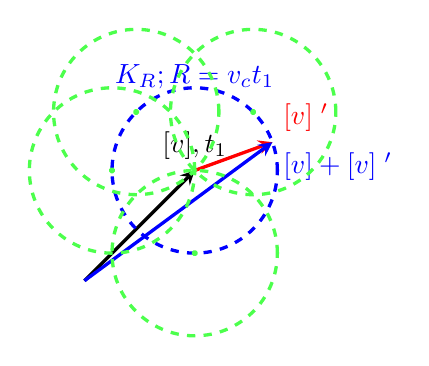
\begin{tikzpicture}[line width = 1.2pt, line join=round,>=stealth, scale=0.7]
\draw [->, visible on=<2->] (-2,-2) -- (0,0) node[anchor=south, visible on=<2->] {$\ortsvektor[v], t_1$}; 
\draw [red,->, visible on=<3->] (0,0) -- (20:1.5) node[anchor=south west, visible on=<3->] {$\ortsvektor[v]\;'$}; 
\draw [blue,->, visible on=<4->] (-2,-2) -- (20:1.5) node[anchor=north west, visible on=<4->] {$\ortsvektor[v]+\ortsvektor[v]\;'$};

\draw[blue, dashed, visible on=<5->] (0,0) circle (1.5);
\onslide<5->{\node[blue] at (0,1.7) {$K_R; R=v_ct_1$};}

\draw[green!70, visible on=<6->] (45:1.5) circle (0.03);
\draw[green!70, dashed, visible on=<6->] (45:1.5) circle (1.5);

\draw[green!70, visible on=<7->] (135:1.5) circle (0.03);
\draw[green!70, dashed, visible on=<7->] (135:1.5) circle (1.5);

\draw[green!70, visible on=<8->] (180:1.5) circle (0.03);
\draw[green!70, dashed, visible on=<8->] (180:1.5) circle (1.5);

\draw[green!70, visible on=<9->] (270:1.5) circle (0.03);
\draw[green!70, dashed, visible on=<9->] (270:1.5) circle (1.5);

\end{tikzpicture}
\end{column}
\begin{column}<+->{.65\textwidth}
  \begin{block}{Huygens-Fresnelsches Prinzip}<10->

    Jeder Punkt einer Wellenfront ist Ausgangspunkt einer neuen Welle, der so genannten \alert{Elementarwelle}.

    Die Elementarwelle hat die gleiche Frequenz und Ausbreitungsgeschwindigkeit wie die Primärwelle.

Die neue Wellenfront ergibt sich durch phasenrichtige Addition -- \alert{Superposition} -- sämtlicher Elementarwellen.

Im dreidimensionalen Raum breiten sich die Elementarwellen \alert{kugelförmig} aus.

{\tiny  Analyse rücklaufenden Elementarwelle:
David A. B. Miller, \enquote{Huygens's wave propagation principle corrected}, Optics Letters 16(18), 1370, 1991.}

\end{block}
\end{column}
\end{columns}

  \end{frame}
  
  
  
\input{finalframe.inc}
   
\end{document}